\documentclass[emulatestandardclasses]{scrartcl}
\usepackage{graphicx}
\usepackage{color}
\usepackage[ngerman]{babel}
\usepackage{hyperref}
\usepackage{fullpage}
\usepackage{calc} 
\usepackage{enumitem}
\usepackage{titlesec}
\newcommand{\todo}[1]{\textcolor{red}{TODO: #1}\PackageWarning{TODO:}{#1!}}
\date{\vspace{-3ex}}
\begin{document}

\title{
	\includegraphics*[width=0.75\textwidth]{ErstesSem/images/hu_logo.png}\\
	\vspace{24pt}
	Hegels Ph"anomenologie des Geistes - ausgew"ahlte Kapitel}
\subtitle{Proseminar SS 17\\
          Dr. Dimitris Karydas\\
          Theologische Fakult"at \\ 
          Humboldt Universit"at zu Berlin}
\author{Lennard Wolf\\
        \small{\href{mailto:lennard.wolf@student.hu-berlin.de}{lennard.wolf@student.hu-berlin.de}}}
\maketitle
\begin{abstract}

Es werden Vorrede, Einleitung und ausgewählte Abschnitte des Werkes gelesen, die mit dessen Anliegen, systematischen Aufbau und der Durchführung einiger entscheidender argumentativer Züge vertraut machen sollten. Vorgesehen sind: die sinnliche Gewissheit, Bewusstsein und Selbstbewusstsein (Herrschaft und Knechtschaft), die absolute Freiheit und das absolute Wissen. Im close reading Verfahren sollte die systematisch geleitete Bewegung, in der der Unterschied des Bewusstseins überwunden wird, an ihren Knotenpunkten nachvollzogen werden.
\end{abstract}
\newpage

\tableofcontents
\listoffigures
\newpage


\section{Einf"uhrungssitzung\\(25.04.17)}

\subsection{Organisatorisches}

\begin{itemize}
  \item Moodle-PW: bewusst (ab 27.04.)
  \item Abgabe: Essay/Protokelle zu insgesamt 10 Seiten
  \item F"ur schein der Teilnahme ist ein Protokoll abzugeben
\end{itemize}

\subsection{Einf"uhrung}

\begin{itemize}
  \item Relevanz? Wird meist fetischistisch behandelt (sowohl positiv und negativ)
  \item Teil des kulturellen/gesellschaftlichen Ged"achtnisses
  \item Ohne Systematik macht Hegel keinen Sinn (Interpretation wird schwer/unm"oglich)
  \item Ziele der Veranstaltung: Fetischmismus soll abgebaut werden (mit Duktus/Systematik vertraut machen), Verst"andnis von Hegels Pr"agung/Relevanz f"ur unsere Zeit, Kontextualisierung des Werks innerhalb der Philosophie-Geschichte (Bez"uge herstellen zum Denken seiner Zeit, und heutigem Denken/Philosophieren)
  \item Einleitung ganz am Anfang geschrieben, Vorrede ganz am Ende
  \item 1806 begonnen, Fr"uhjahr 1807 erschienen, 7 Kapitel (gro"se Kapitel am Anfang, werden immer k"urzer wegen Zeitdruck (Fortbestehen der Uni Jena war unsicher wegen der nahenden Napoleonischen Truppen))
  \item Selbstbewusstsein als Leitfaden zur gesamten Struktur der P.d.G.
  \item S. d. B.s "`Das Zweite Geschlecht"' nach selber Struktur
  \item Bestandsaufnahme "uber die Erfahrung des Bewusstseins ("`Wissenschaft "uber die Erfahrung des Bewusstseins"')
  \item Hegel in einer lebenslangen Entwicklung - \emph{kein} fertiges System $\rightarrow$ kein gro"ses einheitliches System (!)
  \item Erstes gro"ses Buch Hegels (er hat nur wenige geschrieben)
  \item Arbeit am "`System"' ab 1802/03 in zweitem Drittel der Jenaer Zeit (3 Jenaer Systementw"urfe) $\rightarrow$ dadurch bekam er eine Vorstellung davon, was ein philosophisches System ist
  \item Zeit Hegels "`Zeit der gro"sen Systeme"', Beispiel: Festschrift der deutschen Philosophie
  \item Was ist ein System? \emph{Nicht}: Menge an Prinzipien, keine Gliederung von au"sen | \emph{Sondern}: Der Innere Zusammenhang des Ganzen, "`Das Wahre ist das Ganze"', Innere Orientierung am Ganzen, was die Welt am Innersten zusammenh"alt, "`einzige Darstellungsform des \emph{Wahren}"', Wahres nicht als Gegenteil vom Falschen, sondern das Wahre arbeitet aus dem Falschen heraus
  \item Adorno: "`Das Ganze ist das Unwahre"'
  \item Kants Philosophie ist die "`Folie"' auf der Hegel sich abarbeitet, Hauptbezugspunkt ($\rightarrow$ Buch selber zeigt sein kulturelles Ged"achtnis)
  \item Das \emph{Absolute} (Wissen) als Ergebnis des Buchs, "`Kristallnetz der Verkn"upfungen"' (Marx), "`Das Wesen des Denkens"' (\emph{nicht} wo alles gleich ist)
  \item "`Ph"anomenologie des Geistes"' als Einleitung zum System
  \item Philosophie der \emph{Idee}, dessen Tr"ager der Geist ist
  \item "`Realit"at"' ist das was ist, "`Wirklich"' sind die Strukturen dahinter
  \item "`Geist"': Kulturelle Produktion der Menschheitsgeschichte, die Selbstvorstellung des Menschen "uber sich
  \item Wissenschaft ist der Geist, der sich als Weist wei"s - Kulturelle Artefakte sind Versuche der Selbstvorstellung
  \item Junghegelianer, Linkshegelianer verstanden das Buch als Geschichtsphilosophie, Dozent: "uberzeugt von dem Argumenten \emph{dagegen}: 
  \item Buch war laut hegel erst zu dieser Zeit m"oglich (nicht 20 Jahre fr"uher), denn: Protestantismus und franz. Revolution sind Voraussetzung gewesen denn: Freiheit rechtlich kodifizeirt f"ur \emph{alle} $\rightarrow$ Geist thematisiert sich selbst, ohne "au"sere Einfl"usse, totale Selbstbez"uglichkeit
  \item Was nimmt sich das Buch vor? "`Unterschied des Bewusstseins"' "uberwinden (Unterschied zwischen Bildern, die sich das Bewusstsein von der Welt macht, und dem Gegenstand selbst)
  \item Erfahrungsgeschichte--?
  \item Alle Vorraussetzungen immer hinterfragen, "`Wo kommen die her?"'
\end{itemize}

"`\emph{Das Absolute? In unserer Welt?}"'


\section{Einleitung I, S. 53-62\\(02.05.17)}



\subsection{Lekt"urenotizen}

\begin{itemize}
  \item Betrachtung als Werkzeug? Dann ist es mittelbar und bringt nichts!
  \item Es ist nicht m"oglich, sich au"serhalb zu stellen!
  \item Wissen kann nicht begr"undet werden von innen. $\rightarrow$ Widerspruch!
  \item Darstellung des erscheinenden Wissens
  \item Einsicht in die Unwahrheit des erscheinenden Wissens
  \item Hegels Skeptizismus ist nicht als negativ aufzufassen, 
\end{itemize}

\subsection{Einleitung I, S. 53-62}

\begin{itemize}
  \item Einleitung steht vorher durch ihren Bezug zum Werk selber: \emph{Welcher Weg wird weshalb gegangen?}; Zwischen Polemik und Argumentation; Soll Leser in die Schuhe des AUtors stellen, dass das Ende schon bekannt ist!
  \item Vorrede kann auch parallel zum Gesamttext gelesen werden/auf diese kann sich immer
  \item Hegel grenzt sich ab von bisherigem Gedanken der Erkenntnistheorie, die einen Unterschied macht zwischen Methode der Erkenntnis und Erkanntem
  \item Er will "`nat"urliche Erkenntnis"' im Gegensatz zu Kant, der erst den theoretischen Gebrauch der Vernunft kl"aren wollte
  \item Wir \emph{sind} die Wahrnehmung - 
  \item Ziel: Undogmatische (Pr"amissenlose) Philosophie die zum Absoluten f"uhrt
  \item Was ist das Verh"altnis von wahrem und falschem ("`partikularem"') Wissen?
  \item Weg durch die Formen durch die \emph{bestimmte} (nicht abstrakte) Negation, welche keine Verneinung ist, sondern einen neuen Blickwinkel konstituiert durch "`Aufhebung"' des Negierten; 
  \item Nat"urliches Bewusstsein nur denkt Negation las vollst"andige Aufhebung und ist damit einseitig und primitiv
  \item Das Buch soll eine Philosophie der Freiheit begr"unden und stellt seine Einleitung dar (historisch)
  \item "`In der absoluten Idee steckt die absolute Methode"'
  \item Vollst"andigkeit der Form: Gew"ahrleistet durch die gezielte Negation
\end{itemize}

\begin{description}[leftmargin=!,labelwidth=\widthof{\bfseries Erscheinendes Bewusstsein}]
  \item[Die Wirklichkeit] Das was ist, vor der der Betrachtung. ("`Objekt"', muss aber auch als Subjekt gedacht werden!)
  \item[Die Realit"at] Die erscheinende Welt. (Das vom Subjekt wahrgenommene Objekt) |  Erscheinung/Ausdruck des Kreativen Geistes 
  \item[Das Absolute] Die Einheit von Subjekt und Objekt - Wesen und Erscheinung f"allt zusammen (nur im Geist m"oglich, durch den Vollzug der Weltgeschichte). \emph{oder} Struktur der Wirklichkeit (Die Vernunft, Struktur des Denkens). Es gibt nichts au"serhalb des Absoluten.
  \item[Absolutes Wissen] Regeln/Struktur des Denkens, nicht alles Wissen; Dem partikularen/realen Wissen wird immer weiter seine Partikularit"at genommen, bis Subjekt und Objekt ineinanderfallen
  \item[Reales Wissen] vom nat"urlichen Bewusstsein f"ur wirklich gehalten
  \item[Nat"urliche Erkenntnis] 
  \item[Erscheinendes Bewusstsein] 
  \item[Nat"urliches Bewusstsein] Einstellung, die Voraussetzungen eines bestimmten Verfahrens nicht hinterfragt | Jenes das sich als unmittelbar versteht | Dieses gilt es zu bek"ampfen
  \item[Geist] 
  \item[Form] 
  \item[Seele] Schnittstelle von Mensch und Tier
  \item[Ende der Geschichte] ?
  \item[Bestimmte Negation] Wenn man die konkreten Momente benennen kann, die negiert werden m"ussen: Ohne Ma"sstab von au"sen
\end{description}

Pluraletantum

\subsection{Der Aufbau der Phänomenologie des Geistes (Stephan Siemens)}

\begin{itemize}
  \item In einer dialektischen Philosophie, in der der Gedanke der Entwicklung bestimmend ist, verändern sich Inhalt und Form der Philosophie, damit aber auch das Verhältnis der Philosophie zu den Standpunkten, die die Philosophie von außen betrachten und von ihr äußerliche Rechtfertigungen verlangen.
  \item Die Hegelsche Philosophie verbindet das Denken der Totalität mit dem der Entwicklung (Dialketik)
\end{itemize}

\section{Einleitung II, S. 62-68\\(09.05.17)}

\subsection{Sitzung}

\begin{itemize}
  \item Wogegen grenzt sich Hegel ab? Das nat"urliche Bewusstsein/Verfahren
  \item Der Weg (die Bewegung) ist durch das Bewusstsein sein bestimmt
  \item Wissen ist die Seite des Gegenstandes des f"ur das Bewusstsein sein, das an sich ist die Wahrheit, das an sich ist auch f"ur es! 
  \item Ma"stab zur "Uberpr"ufung des gegenstands und sich selber wird vom Bewusstsein selbst gestellt; Bewusstsein seiner selbst
  \item Gegenstand (an sich) und Begriff (f"ur es) werden konstant gepr"uft! $\rightarrow$ Erfahrung
  \item Wissen: Was das Bewusstsein meint zu wissen... ("`Es ist 10 Uhr"')
  \item Wirklichkeit: Die tats"ahliche Uhrzeit.
  \item Wahrheit: bestimmte Negation das Wissen, ver"andert das WIssen, das Bewusstsein \emph{kann} das nicht merken, "`Wir"' schon
  \item logische Reduplikation
  \item "`Wir"' gucken dem Bewusstsein "uber die Schulter
  \item "`Wir"' wird mit dem Bewusstsein zusammenfallen, wenn "`es"' sich in "`unsere"' Position erhoben hat
  \item 1.: Das "`an sich f"ur es"', 2.: das "`an sich"', 3.: "`an sich f"ur uns"'
  \item Begriff: 
  \item "`Wir"': Auf dem STandpunkt des Ergebnisses des Buches; vollziehen die Erfahrung nach, das Bewusstsein "andert sich und damit das Bild (Wissen prallt auf Wahrheit), dabei "andert sich der Gegenstand, aber das Bewusstsein kann das nicht merken
  \item Das Bewusstsein verzweifelt weil es das Wissen updatet, der Gegenstand sich ver"andert, und das immer so weiter geht
  \item Wenn man denkt, man habe einen Begriff (in diesem Buch) verstanden, dann hat man ihn/es nicht verstanden.
\end{itemize}

\section{Sinnliche Gewi"sheit, S. 69-78\\(16.05.17)}

\subsection{Lekt"urenotizen}

\begin{itemize}
  \item Sinnliche Gewi"sheit: Erkenntnis deren konkreter Inhalt unendlich zu sein scheint, da er immer weiter teilbar ist 
  \item Sinnlichem Wissen ist das Wesentliche, dass die Sache \emph{ist}; Sinnliche Gewi"sheit ist unmittelbare Beziehung zwischen Einzelnem und Sache oder Bewu"stsein (Ich, reiner dieser)
  \item Das Allgemeine ist etwas das durch Negation ist; es ist das Wahre der sinnlichen Gewissheit -- WARUM?
  \item Wir \emph{meinen} das sinnliche Sein wenn wir sprechen, doch wir k"onnen immer nur das Allgemeine sagen
  \item Das Allgemeine ist nur durch einfaches Dieses vermittelbar
  \item Ist das Dies an sich allgemein?
  \item Vermittlung ist Negation
\end{itemize}
\section*{R"uckblick auf die Einleitung}
%\large
\begin{description}[leftmargin=!,labelwidth=\widthof{\bfseries Unterschied des Bewusstseins}]
  \item[Bewusstsein] Prozess der Umkehrung/Selbstpr"ufung des Bewusstseins, sowie seines Bewusstseinsgegenstandes, wodurch das Bewusstsein etwas anderes wird. Und diese Ver"anderung ist die Erfahrung. So bestreitet es einen Weg, "uber welchen es zur 	Selbstthematisierung kommt.
  \item[\emph{An sich f"ur es}] Das Bild das sich das Bewusstsein von etwas macht, sein Wissen. "Uber dieses kommt das Bewusstsein zur Erfahrung. Bild vom Gegenstand entspricht nicht dem, wie er f"ur sich selbst ist (Wahrheit).
  \item[Wir] Instanz des Autors/Lesers, die dem Bewusstsein "uber die Schulter schaut und "`redupliziert"' die Erfahrung des Bewusstseins im Buch/Lesen.
  \item[Unterschied des Bewusstseins] Unterschied zwischen dem \emph{an sich f"ur es} (Wissen) und dem, womit das Bewusstsein dieses Wissen vergleicht (Wahrheit).
  \item[Vollst"andigkeit der Form] Wird erreicht dadurch, dass durch die doppelte bestimmte Negation alles einseitige Wissen "uber den Gegenstand verworfen wird.
\end{description}


Die "`Ph"anomenologie des Geistes"' bestreitet einen Weg "uber welchen der theoretische und praktische Bezug des Bewusstsein zur Welt hin zum Selbstbezug vollst"andig res"umiert wird.

%\section*{Vortrag}


\section*{Sitzung}

\emph{Sagen wir, wir kaufen Hegel das zur sinnlichen Gewissheit Geschriebene ab, was haben wir gewonnen?}

Wir haben die \emph{Form der Wahrnehmung/des Aufzeigens} erfahren. Wir haben das abstrakte Allgemeine kennengelernt, von welchem das Bewusstsein beim Erkennen immer anf"angt. Das Bewusstsein nimmt zuerst unmittelbar (sinnlich) wahr, und (erst) wenn es etwas aufzeigen will (zum Beispiel beim Begreifen des Gegenstandes), muss es auf das Allgemeine rekurrieren. Wir haben von der Wahrhaftigkeit des Allgemeinen erfahren und seine Beziehung zum einfachen Einzelnen verstanden.\newline

\noindent \emph{Ist das, was Hegel macht, \emph{neu}?}

Das \emph{Neue} des Buches ist, dass die bisherigen Resultate, zu denen die Menschheitsgeschichte schon gekommen ist, sei es durch hohe Philosophie oder durch allgemeines Gedankengut, auf neue Art und Weise zusammen gestrickt werden -- eine "`Reduplikation der Erkenntnisee"'. Hegel benutzt zu diesem Zwecke Terminologie genau wie die gemeine Sprache sie benutzt.\newline

\noindent \emph{Dreierlei muss zum Verst"andnis eines jeden Abschnittes des Buches erkannt werden:} 

Mit welchem \textbf{Meinen} (\emph{Wissen}) wird begonnen, welche \textbf{Schritte} werden mit diesem Wissen durchgef"uhrt, und zu welcher \textbf{Erkenntnis} wird gelangt.\newline

"`\emph{Vergleichen wir das Verh"altnis, in welchem das Wissen und der Gegenstand zuerst auftrat, mit dem Verh"altnisse derselben, wie sie in diesem Resultate zu stehen kommen, so hat es sich umgekehrt. Der Gegenstand, der das Wesentliche sein sollte, ist nun das Unwesentliche der sinnlichen Gewi"sheit, denn das Allgemeine, zu dem er geworden ist, ist nicht mehr ein solches, wie er f"ur sie wesentlich sein sollte, sondern sie ist itzt in dem Entgegengesetzten, n"amlich in dem Wissen, das vorher das Unwesentliche war, vorhanden.}"'\newline


%\noindent \emph{Wie verh"alt es sich in diesem Kapitel?} 

\begin{description}[leftmargin=!,labelwidth=\widthof{\bfseries Negation der Negation}]
  \item[Meinen] Wissen als Wissen des Unmittelbaren, des Seienden, dessen was uns darbietet. ("`Jetzt ist das Sein der Nacht"')
  \item[Negation] Wenn das Bewusstsein von etwas Seiendem sprechen wollen, dann spricht es automatisch vom Allgemeinen, auch wenn es das Seiende meint. Durch Kenntnis des Prozesses der Ver"anderung wird das Seiende als sekund"ar erkannt. $\rightarrow$ Wissen als Wissen des abstrakt Allgemeinen ("`Jetzt ist ein Allgemeines"')
  \item[Negation der Negation] Das Jetzt ist aber bei jeder Aufzeigung ("`Jetzt ist 12 Uhr"') schon wieder vergangen, und also nur \emph{gewesen}. Aber wenn es "`nur"' \emph{gewesen} ist, dann \emph{ist} es nicht, und darum ging es uns aber. $\rightarrow$ "`Das Jetzt \emph{ist}"'.
  \item[Erkenntnis] Allein durch das Reflektieren "uber das Einfache und das daraus resultierende Erfahren, dass es ein Allgemeines ist, kommen wir zum wahrhaften Einfachen, "`welches im Anderssein bleibt, was es ist"' 
\end{description}

"`\emph{Es erhellt, da"s die Dialektik der sinnlichen Gewi"sheit nichts anders als die einfache Geschichte ihrer Bewegung oder ihrer Erfahrung, und die sinnliche Gewi"sheit selbst nichts anders als nur diese Geschichte ist. Das nat"urliche Bewu"stsein geht
deswegen auch zu diesem Resultate, was an ihr das Wahre ist, immer selbst fort, und macht die Erfahrung dar"uber; aber vergi"st es nur ebenso immer wieder, und f"angt die Bewegung von vorne an. }"'\newline

Es bleibt nun zu kl"aren, was die \emph{Form der Wahrnehmung} ist, d.h. was es bedeutet, etwas wahrzunehmen.

\section*{Offene Fragen}

\begin{itemize}
  \item Ist Sprache sekund"ar? Wie steht sie in Beziehung mit dem Bewusstsein?
  \item Zerbricht alles in diesem Buch, wenn auch nur an einer Stelle ein Fehlschluss gemacht wird? (W"are Fehlschluss nicht nur ein weiterer Schritt im Weg zur Erkenntnis? Es gibt nicht "`das System"'. Aber wie kann dann "uberhaupt Kritik an Hegel ge"ubt werden?)
\end{itemize}

\subsection{Fragen}

\begin{itemize}
  \item Popper: reinforced dogmatism (\url{https://de.wikipedia.org/wiki/Immunisierungsstrategie#Doppelt_verschanzter_Dogmatismus})
  \item Bereits Arthur Schopenhauer schrieb 1830, Dialektik sei die Kunst, in einem Disput immer Recht zu behalten.
  \item Ist nicht das partikulare Sein eines Gegenstands die Wahrheit der sinnlichen Gewissheit? was ist Wahrheit der sinnlichen Gewissheit? 
  \item ist nicht das allgemeine schon vermittelt? als allgemeines f"ur mich, wenn doch aber die sinnliche Gewissheit unmittelbar ist?
  \item Gibt es das Hier? Nein!
  \item Ist das Dies an sich allgemein?
\end{itemize}

Worum ging es in der Einleitung? Worum wird es gehen, wenn wir von Erfahrung des Bewusstseins sprechen? Was erf"ahrt das Bewusstsein? Worin besteht es? Wie kommt es zu Erfahrung? Prozess der Umkehrung/Selbstpr"ufung des Bewusstseins, sowie seines Bewusstseinsgegenstandes, wodurch das Bewusstsein etwas anderes wird. Und diese Ver"anderung ist die Erfahrung. So bestreitet es einen Weg, "uber welchen es zur Selbstthematisierung kommt. 

Wir k"onnen das Buch nur aus dem Standpunkt der heutigen Zeit lesen. 

In der Natur kommt das Negative nicht über sich selbst hinaus, sondern bleibt im Endlichen gefangen. Das Samenkorn geht auf, wächst zu einem Baum, der Baum stirbt und hinterlässt das Samenkorn; Anfang und Ende fallen zusammen. In der Philosophie des Geistes gibt es eine Entwicklung des Begriffs – die Geschichte. Der Begriff kommt zu sich selbst. Die Negation ist hier nicht zirkulär, sondern treibt den Fortschritt spiralförmig in eine Richtung hin. 


\section{Sinnliche Gewi"sheit, S. 69-78\\(16.05.17)}

\subsection{Gefundenes}

The Yin-Yang model and the Hegelian model [as suggested in the highlighted part of the brief introduction to Hegel’s relevant thought in the appendix below] of interaction have their common points in some respects and distinctive in others. (1) Both models highlight the universal existence of two correlative contraries, yin and yang or thesis and anti-theisis. (2) Both emphasize that the relations  between the contaries are interdependent and interactional. (3) The interactional relation is considered fundamental since the interaction of the two contraries constitutes the ultimate source and final pushing force for the transformation and development of all things in the universe. (4) The independent relation is dynamic rather than static. (5) As far as the dynamic development is concerned, both stress reaching equilibrium or a kind of (dynamic) balance. However, on the other hand, there are some interesting distinctions in regard to focus and emphasis. (1) As far as their emphasis on the interaction between the contraries is concerned, the Yin-Yang way emphasizes cooperation within, while the Hegelian dialectical way stresses opposition without. (2) Insofar as both emphasize equilibrium, the Yin-Yang way endeavors to reach harmony within the Yin-Yang unity through complementarity, while the Hegelian way endeavors to reach synthesis without or beyond thesis-antithesis through sublation. 
 
Objective reality is a synthetic construct, dealing with a hypothetical universalization of multitude of subjective realities. 
 
Wir k"onnen zur Erkenntnis nur durch die Negation kommen, da diese die Grenzziehung darstellt, ohne die ein Begriff nicht m"oglich ist.


\subsection{Lekt"urenotizen}

\begin{itemize}
  \item Der Verstand ist ("`im Wahrnehmen"'(?)) nur das konstante Spiel zwischen Einzelnem und Allgemeinem -- Er springt zwischen zwischen Wissen und Unwissen 
  \item Um hinter den Vorhang zu schauen müssen wir selber hinter den Vorhang gehen und was wir dann da finden sind nur wir selber.
  \item Die Weisen des Bewusstseins: das Meinen, das Wahrnehmen und der Verstand
  \item Kontext f"ur n"achstes Kapitel: Unser Ziel ist es zu erkennen was das Bewusstsein wei"s, indem es sich selbst wei"s 
\end{itemize}

\begin{description}[leftmargin=!,labelwidth=\widthof{\bfseries Negation der Negation}]
  \item[Meinen] Vorhandenes Wissen
  \item[Wahrnehmen] Unmittelbares Wissen
  \item[Verstand] selbstvermittelndes; ist im Innern leer
\end{description}

\begin{figure}[h]
	\centering
	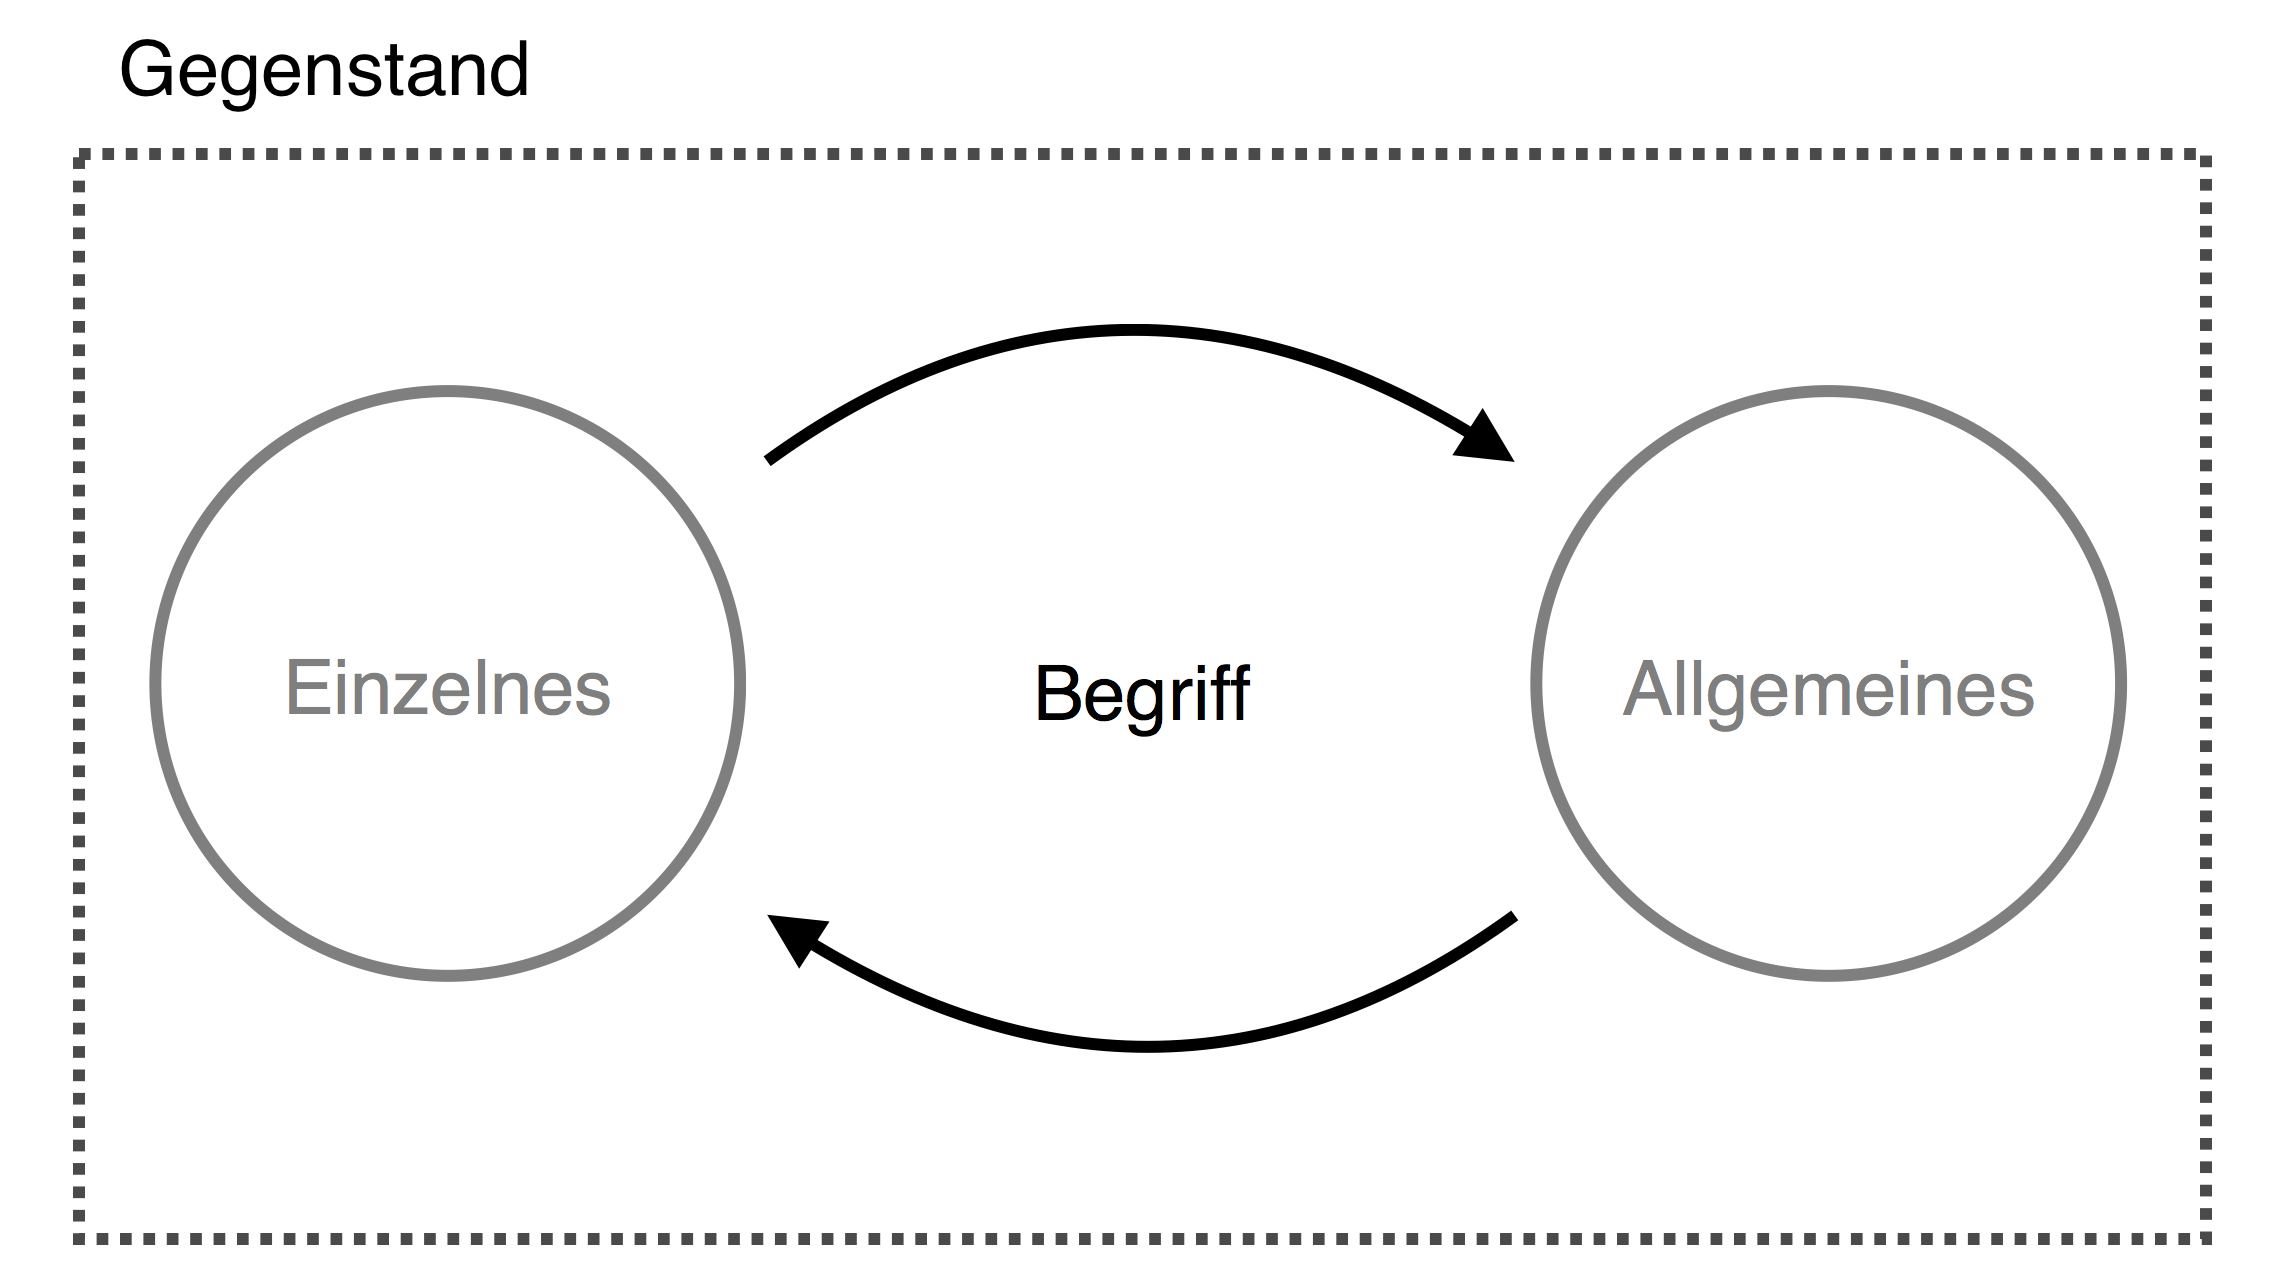
\includegraphics[width=0.5\textwidth]{images/gegenstand}
	\caption{Gegenstand und Begriff sind eins.}
	\label{fig:gegenstand}
\end{figure}

\begin{itemize}
  \item Das Wissen ist zugleich Begriff und Gegenstand (wie alles). Siehe Abbildung \ref{fig:gegenstand}.
  \item Thema: das Wissen von sich selbst
  \item das "`Andere"' fehlt nun, doch bestimmte Momente sind noch vorhanden
  \item Das Hauptmoment des Andersseins ist verloren, denn: Selbstbewusstsein ist die bewegungslose Tautologie "`Ich bin Ich"'
  \item das Meinen, das Wahrnehmen und der Verstand...?
  \item Das an sich ist die Einheit des Unterschiedenen (!, siehe Abbildung \ref{fig:gegenstand}.)
  \item Das Wesen des Individuellen ist das Allgemeine
  \item Die "`Fl"ussigkeit"' (Struktur) ist unterschiedslos!
  \item Leben ist das sich entwickelnde, und seine Entwicklung aufl"osende, und in dieser Bewegung sich einfach erhaltende Ganze.
  \item Sinnliche Gewissheit - Wahrnehmung - Selbstbewusstsein - Vernunft
  \item $\rightarrow$ Jeden Absatz in einem Satz!
\end{itemize}

\subsubsection{Unterschiedenes und Ununterschiedenes}\label{sec:leben}

\begin{description}[leftmargin=!,labelwidth=\widthof{\bfseries Neg. d. Neg.}]
  \item[Meinen] Die "`fl"ussige Substanz"'\footnote{Dieser abstrakte Begriff wird wohl im weiteren Verlauf durch "`Geist"' ersetzt.} als ununterschiedene Einheit, als "`reine achsendrehende Bewegung"', als "`absolutunruhige Unendlichkeit"' (das \emph{Ansich}).
  \item[Negation] Entzweiung zu selbst"andigen Gestalten als Bestimmte  (das \emph{Andere f"ur sich}) | Aber: die Gestalten bestehen aus der "`Substanz"' und sind so immer an diese gebunden.
  \item[Neg. d. Neg.] Die "`fl"ussige Substanz"' als ununterschiedene Einheit, die aber der unendliche Unterschied ist.
  \item[Erkenntnis] Das Ganze und das Individuelle bedingen einander. Das Leben ist f"ur das Selbstbewusstsein die Einheit, oder Gattung.
\end{description}

\subsubsection{Selbstbewusstsein}

\emph{"`Nunmehr aber ist dies entstanden, was in diesen fr"uhern Verh"altnissen nicht zustande kam, n"amlich eine Gewi"sheit, welche ihrer Wahrheit gleich ist, denn die Gewi"sheit ist sich selbst ihr Gegenstand, und das Bewu"stsein ist sich selbst das Wahre."'} (S. 120)


Da in den "Uberlegungen dieses Abschnitts das Bewusstsein sich selbst thematisiert, f"allt zu allererst auf, dass es gleichzeitig Bewusstsein und Gegenstand zugleich ist. So ist der Gegenstand dem Bewusstsein hier als Gewissheit aber nicht von der Wahrheit getrennt.

\begin{description}[leftmargin=!,labelwidth=\widthof{\bfseries Neg. d. Neg.}]
  \item[Meinen] Selbstbewusstsein als unmittelbares Bewusstsein vom \emph{ununterschiedenen Ich}.
  \item[Negation] Selbstbewusstsein als Bewusstsein von sich selbst als \emph{Anderem} Sein. | Aber: der Unterschied \emph{ist} nicht, "`Ich bin Ich"' ist bewegungslose Tautologie: hier ist keine sinnliche Wahrnehmung, hier ist kein Proze"s.
  \item[Neg. d. Neg.] Selbstbewusstsein als unmittelbares Bewusstsein vom ununterschiedenen Ich, das eine unerf"ullte Begierde danach hat, wahrgenommen zu werden.
  \item[Erkenntnis] Befriedigung der Einheit seiner Selbst als unmittelbares Bewusstsein in einem Anderssein muss durch ein anderes Bewusstsein erreicht werden.
\end{description}

\emph{"`Indem ein Selbstbewu"stsein der Gegenstand ist, ist er ebensowohl Ich, wie Gegenstand."'} (S. 127)

\emph{"`Das Selbstbewu"stsein stellt sich hierin als die Bewegung dar, worin dieser Gegensatz aufgehoben, und ihm die Gleichheit seiner selbst mit sich wird."'} (S. 122)

\emph{"`Das Selbstbewu"stsein erreicht seine Befriedigung nur in einem andern Selbstbewu"stsein."'} (S. 126)

\subsection{Sitzung}

\subsubsection{Vorbemerkungen}

\begin{itemize}
  \item Quintessenz des ersten Abschnitts: Das Bewusstsein beim allerfundamentalsten Akt des Beziehens aus der fundamentalsten unmittelbarsten sehr schnell zum Schluss kommt, dass es sich immer auf das Allgemeine bezieht, auf eine Abstraktion, um zu irgendeiner Aussage kommen zu k"onnen!
  \item Partikulare Aussagen die man trifft sind nicht auf Abstraktionen reduzierbar, d"urften sie auch nicht, denn ansonsten 
  \item Baumann Interpretation von Hegel
  \item Es lohnt sich zum Verst"andnis immer auch den Anfang des n"achsten Kapitels zu lesen, da dort in verdichteter Form nochmal der derzeitige Standpunkt aufgezeigt wird. 
  \item Zur Einsicht kommt es erst am Ende
\end{itemize}

\subsubsection{Wahrnehmung}

\begin{itemize}
  \item Abfolge von Gestalten des Bewusstseins, die dadurch zustande kommen, dass das Bewusstsein feststellt, dass es einen Unterschied gibt zwischen seinem Wissen und der Wahrheit 
  \item Wahrheit ist das was erreicht wird nach Pr"ufung des Wissens durch wahrgenommenes, und sie wird dann das neue Wissen, und so kann sie niemals festgehalten werden!
  \item Irgendwo muss das Bewusstsein anfangen: 
  \item Jede Erfahrung die ein Bewusstsein macht ist eine Selbstver"anderung
  \item Gestalten des  Bewusstseins: Formen die das Bewusstsein annimmt, immer eine neue, wenn es merkt, dass die Wahrheit nicht dem Wissen entspricht
  \item Sinnliche Gewissheit: Gegenst"ande sind uns in der form der sinnlichen Wahrnehmung gegeben.
  \item Form der sinnlichen Wahrnehmung ist nicht festzuhalten, es geht um die Form/Gestalt in denen Sie wie ein Ding mit Eigenschaften erscheint
  \item Der Allgemeine Bezug macht keinen Sinn ohne Verbindung zum Konkreten!
  \item Wir wollen Form der Wahrnehmung problematisieren: die Allgemeine Form der Wahrnehmung besteht darin, dass unterschieden wird zwischen einem Wahrnehmenden und einem Wahrgenommenen. 
  \item "`Wir nehmen \emph{f"ur wahr}."'
  \item Gang durch die Verkettung der Notwendigkeiten folgt zur absoluten Erkenntnis (?)
  \item Die Bewegung, wie der Gegenstand sind dem Wesen nach das selb. wobei der Gegenstand das zusammengefasst sein der Momente ist
  \item Warum haben wir keine unmittelbare Gewissheit? Weil diese nicht festzuhalten w"are, alles ist akzidentiell, wir k"onnen nur das Allgemeine/Wesentliche festhalten -- drum muss dieses konkreter werden
  \item Wesentlich f"ur die Wahrnehmung ist die Negation: denn es ist wichtig dass wir das Mannigfaltige wahrnehmen, im Bezug zum Konkreten
  \item Bewusstsein ist nunmal im konstanten Prozess, ist nicht festzuhalten, und so "andert sich konstant aller Sinn
  \item Gegenst"ande: es bleibt nichts "ubrig. Es gibt Dingheit, aber das partikulare Ding l"asst sich \emph{ganz} aber nicht greifen (Kant)
  \item Wie bilden wir unsere Meinung/Sicht auf die Gegenst"ande? -- Reflexion: Das Ding soll mit seinen wahrgenommen Eigenschaften verschmelzen
  \item "`Reflexion"': Der Akt einer Unterscheidung (zwischen Bewusstsein und Gegenstand) | nicht zu trennen vom Gegenstand, nicht blo"s \emph{denken}, sondern \emph{denken "uber}
  \item Gegenstands Wahrnehmung ist eine konstante Vermittlung zwischen Wahrnehmung und Allgemeinem Bild
  \item Zum n"achsten mal: Wahrnhemung und T"auschung lesen!
  \item Begierde: Jede Bezugnahme ist auch eine Bezugnahme auf uns selbst.
\end{itemize}


\subsubsection{Kraft und Verstand}

\begin{itemize}
  \item Kraft: 
  \item Kraft"au"serung: 
  \item Einheit von Bewusstsein: Erkenntnis dass wenn wir uns auf die Welt bezehne, im Grunde wir uns selbst thematisieren. Das was dahinter steckt sind wir selbst -- nicht dass die Welt verschwinden w"urde wenn wir nicht da w"aren, nur dass der Bezug zur Welt nur Sinn macht, wenn wir auf uns selbst Bezug genommen haben
  \item Intersubjektivit"at: Bewusstsein ist kein Individuum, sondern im Bezug auf andere
  \item 
\end{itemize}

"`Man braucht das du, nat"urlich, sie werden gerade besch"amt."'

\newpage
\section{"Uber den Professor}
Prof. Mustermann ist..


%\begin{figure}[h]
%	\centering
%	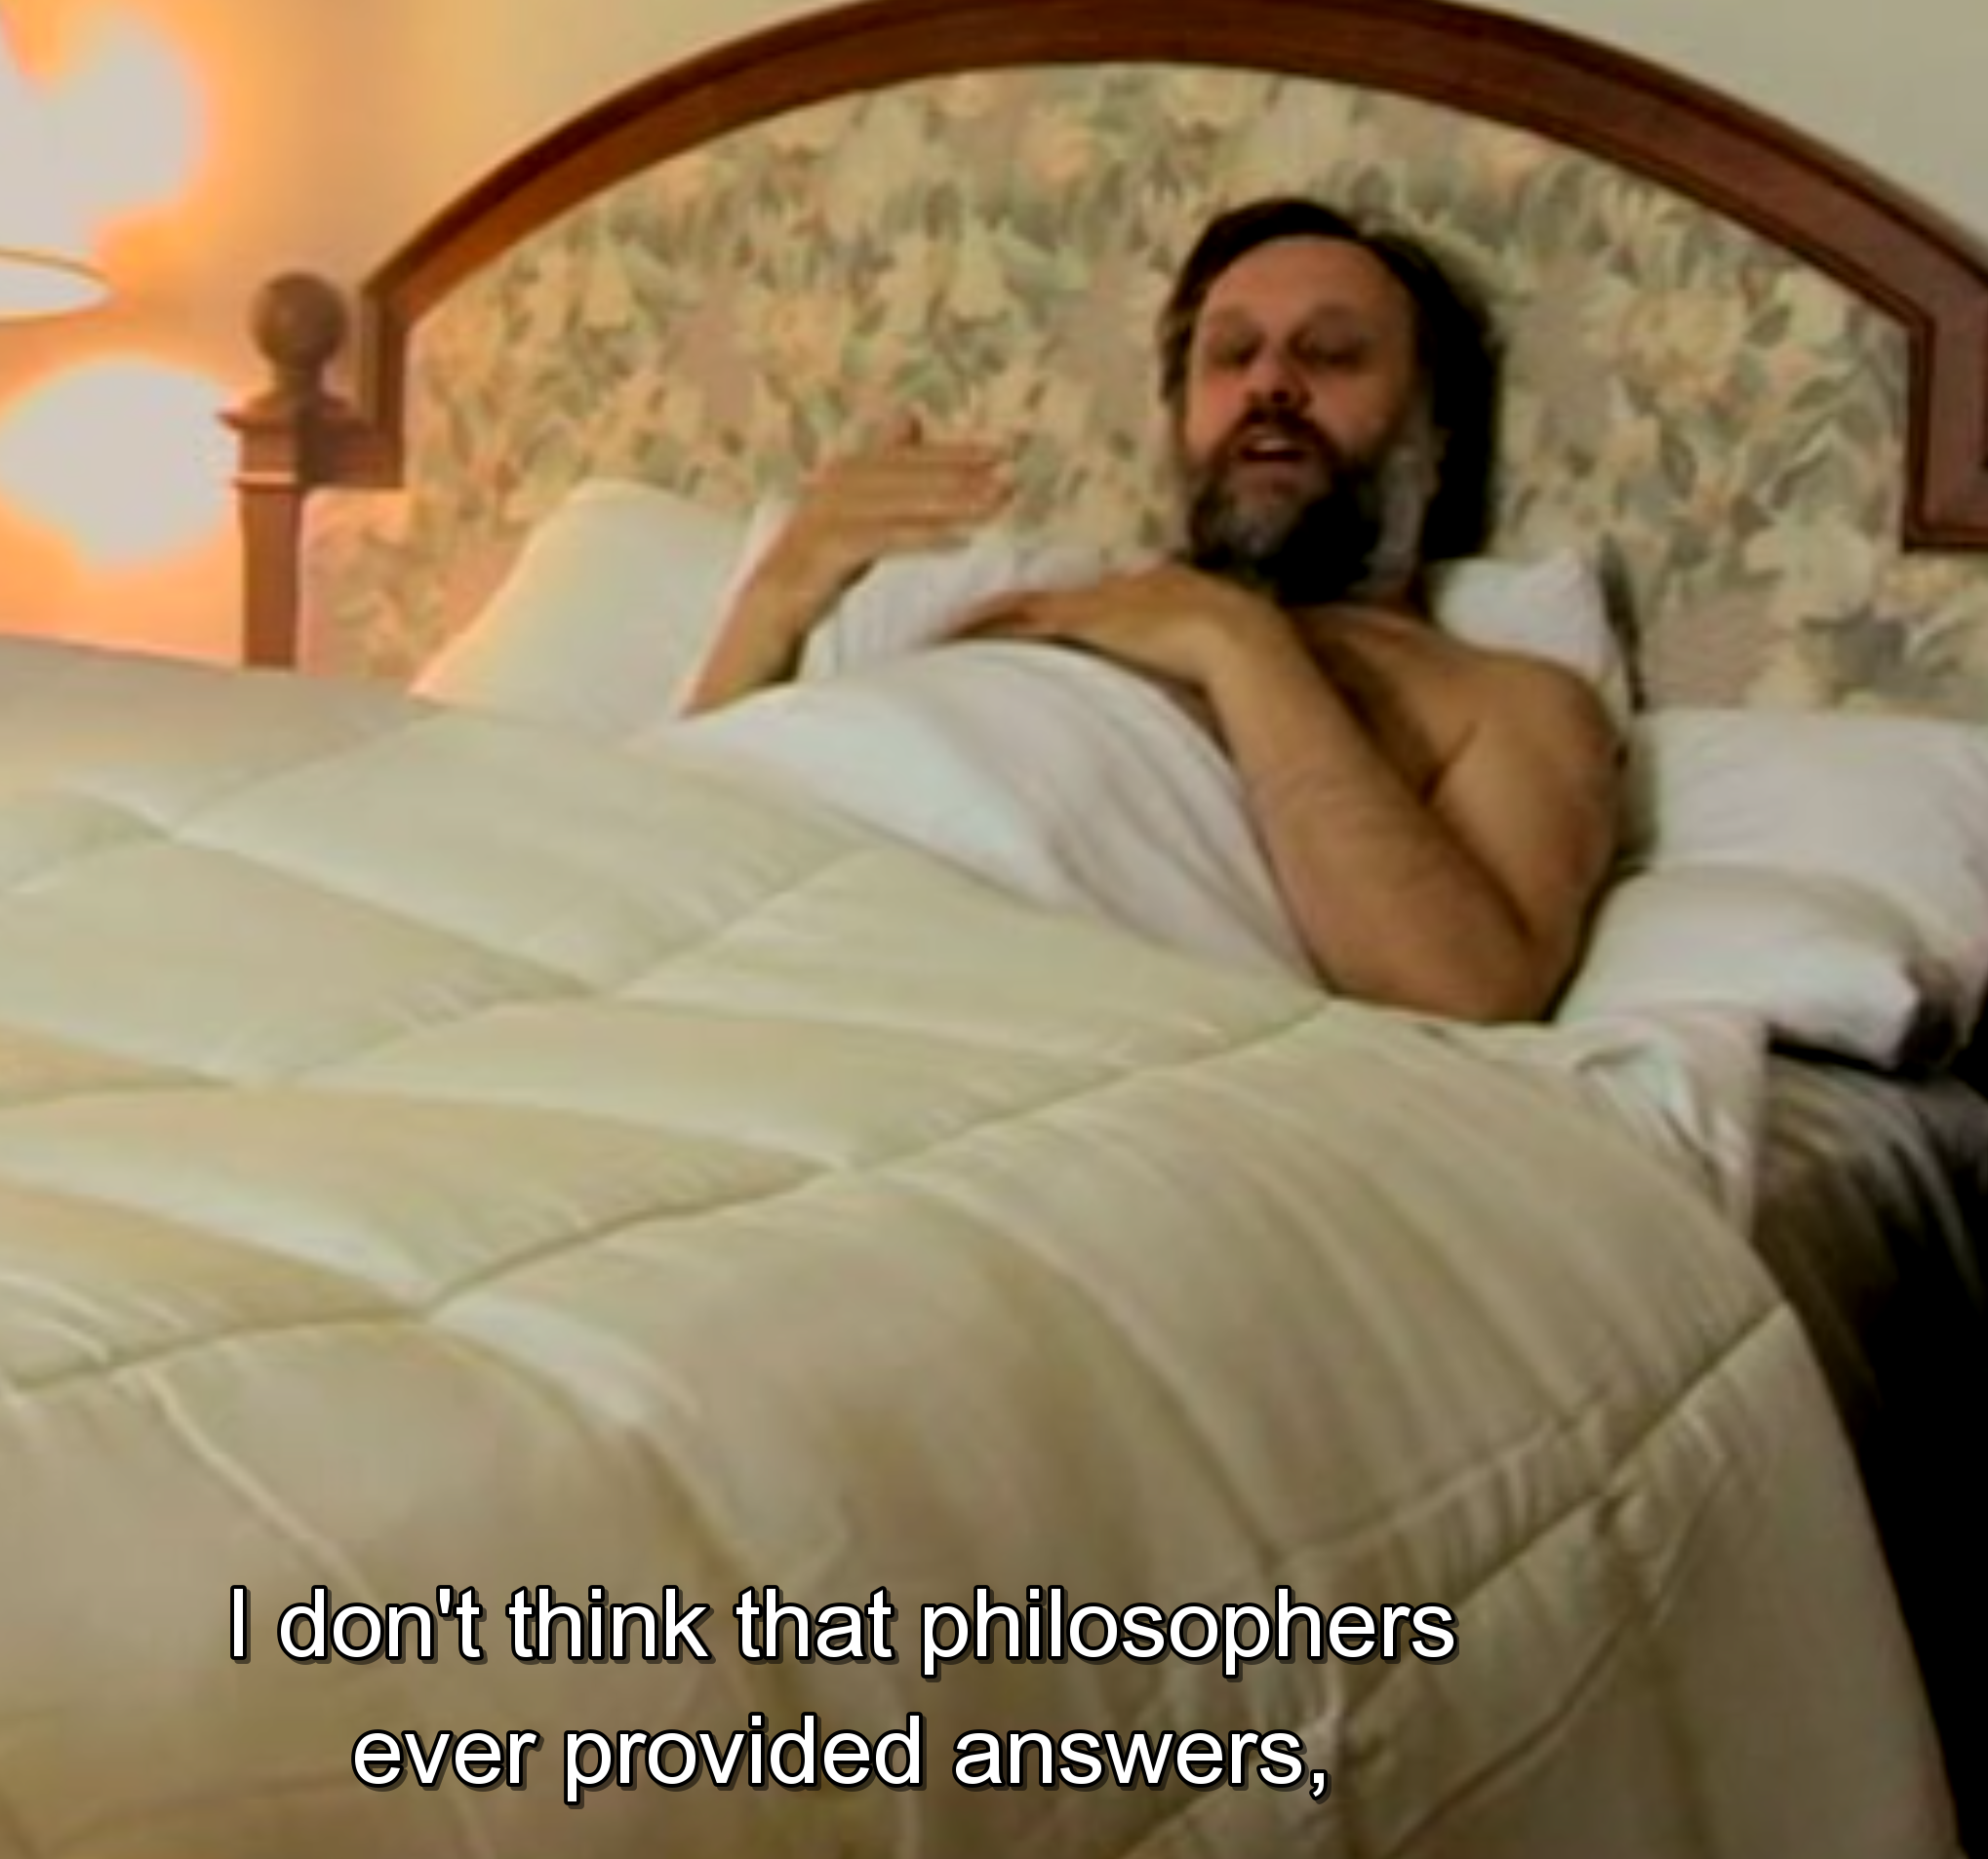
\includegraphics[width=0.5\textwidth]{images/template.png}
%	\caption{Template Bild}
%	\label{fig:template}
%\end{figure}

\end{document}
